\chapter{Ondes électromagnétiques}

%%%%% /!\ PROFESSEURS : Quid des singularités pour l'espace? Nous parlons d'un espace vide de charges et de courants en ce qui concerne les ondes EM mais pourquoi ? 
%%%%% Comment se figurer un tel espace? Aussi, il semble que les ondes EM se propagent très bien malgré la présence de charges ou de courants?  ==>> CLARIFICATION NECESSAIRE

Dans cette section, nous allons aborder une partie primordiale du cours qui concerne les ondes électromagnétiques. \\
\textit{Qu'est ce qu'une onde électromagnétique}? Nous pouvons définir une onde EM comme la \textbf{propagation d'un signal} à travers l'espace; 
ce signal correspond à une \textbf{\textit{variation couplée}} d'un champ électrique et d'un champ magnétique.  Ce signal se transmet à une vitesse qui est propre au milieu traversé comme nous le verrons à la section suivante. 
Pour l'instant, nous allons partir des équations de Maxwell pour aboutir sur l'équation définissant les ondes EM. Pour rester relativement global tout en simplifiant parfois les choses, nous approcherons le problème de manière générale et traiterons ensuite en profondeur des cas particuliers. 
\footnote{Théorie provenant conjointement des slides et de \textit{wikipédia} : \url{https://fr.wikipedia.org/wiki/Établissement_de_l\%27équation_de_propagation_à_partir_des_équations_de_Maxwell}}

%\subsection{Formulation générale et équation d'Alembert}

\section{Notions et notations}

Cette sous-section vise à introduire les notions mathématiques et physiques dont nous aurons besoin afin d'arriver à nos fins. 
%\begin{fullwidth}
%	\begin{center}
%		
%		\begin{tabular}{|c|c|c|}
%			
%			\hline
%			
%			1 & Champ électrique & $\vec{E}(x,y,z,t) = E_{x}(x,y,z,t) \hat{x} + E_{y}(x,y,z,t) \hat{y} + E_{z}(x,y,z,t) \hat{z}$ \\
%			
%			\hline
%			
%			2 & Champ magnétique d'excitation &  $\vec{H}(x,y,z,t) = H_{x}(x,y,z,t) \hat{x} + H_{y}(x,y,z,t) \hat{y} + H_{z}(x,y,z,t) \hat{z}$ \\
%			
%			\hline 
%			
%			3 & \textit{\textbf{Laplacien}} vectoriel & $\Delta \vec{R} = \nabla^{2}(R_{x}(x,y,z,t) \hat{x} + R_{y}(x,y,z,t) \hat{y} + R_{z}(x,y,z,t) \hat{z}) $\\
%			
%			\hline
%			
%			4 & Propriété & $\nabla \times (\nabla \times \vec{R}) = \nabla(\nabla \cdot \vec{R}) - \Delta \vec{R} $\\
%			
%			\hline
%			
%			5 & Première équation de \textit{\textbf{Maxwell}} & $\nabla \cdot \vec{E} = \frac{\rho}{\epsilon}$ \\
%			
%			
%			6 & Troisième équation de \textit{\textbf{Maxwell}} & $\nabla \times \vec{E} = - \mu \frac{\partial \vec{H}}{\partial t}$ \\
%			
%			
%			7 & Quatrième équation de \textit{\textbf{Maxwell}} & $\nabla \times \vec{H} =  \vec{J} + \epsilon \frac{\partial \vec{E}}{\partial t}$ \\
%			
%			\hline
%			
%		\end{tabular}
%		
%	\end{center}
%\end{fullwidth}
\begin{enumerate}
\item{Champ électrique} \begin{center}$\vec{E}(x,y,z,t) = E_{x}(x,y,z,t) \hat{x} + E_{y}(x,y,z,t) \hat{y} + E_{z}(x,y,z,t) \hat{z}$\end{center} 
\item{Champ magnétique d'excitation } \begin{center}$\vec{H}(x,y,z,t) = H_{x}(x,y,z,t) \hat{x} + H_{y}(x,y,z,t) \hat{y} + H_{z}(x,y,z,t) \hat{z}$\end{center} 
\item{\textit{\textbf{Laplacien}} vectoriel} \begin{center} $\Delta \vec{R} = \nabla^{2}(R_{x}(x,y,z,t) \hat{x} + R_{y}(x,y,z,t) \hat{y} + R_{z}(x,y,z,t) \hat{z}) $\end{center} 
\item{Propriété} 
\begin{center}$\nabla \times (\nabla \times \vec{R}) = \nabla(\nabla \cdot \vec{R}) - \Delta \vec{R} $\end{center} 
\item{Première équation de \textit{\textbf{Maxwell}}} 
\begin{center}$\nabla \cdot \vec{E} = \frac{\rho}{\epsilon}$\end{center} 
\item{Troisième équation de \textit{\textbf{Maxwell}}}
\begin{center}
$\nabla \times \vec{E} = - \mu \frac{\partial \vec{H}}{\partial t}$
\end{center} 
\item{Quatrième équation de \textit{\textbf{Maxwell}}} \begin{center} $\nabla \times \vec{H} =  \vec{J} + \epsilon \frac{\partial \vec{E}}{\partial t}$\end{center} 
\end{enumerate}
\section{Développement par combinaison}

Maintenant que nous avons introduit les différentes données de notre développement, nous pouvons  commencer à combiner les équations. 
Si nous dérivons la quatrième équation de Maxwell (7) par rapport au temps, nous pouvons écrire\sidenote{Grâce au théorème de \textbf{Schwarz}.} 

\[ \frac{\partial (\nabla \times \vec{H})}{\partial t} = \nabla \times \frac{\partial \vec{H}}{\partial t} = \frac{\partial(\vec{J} + \epsilon \frac{\partial \vec{E}}{\partial t})}{\partial t} \]

Nous nous rendons rapidement compte que cette dérivée partielle peut également faire apparaitre la troisième équation de Maxwell : 

\[ \nabla \times \frac{\partial \vec{H}}{\partial t} = -\frac{1}{\mu}( \nabla \times (\nabla \times \vec{E}))\]

En recombinant rapidement ces deux équations, nous pouvons mettre en exergue la relation suivante : 

\[-\mu(\frac{\partial \vec{J}}{\partial t} + \epsilon \frac{\partial^{2} \vec{E}}{\partial t^{2}}) = \nabla \times (\nabla \times \vec{E})\]

Etant donnée la propriété\sidenote{Que nous n'allons pas démontrer car cette démonstration sort du cadre du cours.} (4 ème entrée du tableau) concernant le rotationnel du rotationnel, 
nous pouvons écrire la dernière équation sous une forme ne faisant plus intervenir le rotationnel : 

\[ \Delta \vec{E} - \mu \epsilon  \frac{\partial^{2} \vec{E}}{\partial t^{2}} = \mu \frac{\partial \vec{J}}{\partial t} + \nabla(\nabla \cdot \vec{E}) \]

La première équation de Maxwell nous permet d'affiner notre équation d'onde en jouant avec les densités de charge : 

\[ \Delta \vec{E} - \mu \epsilon  \frac{\partial^{2} \vec{E}}{\partial t^{2}} = \mu \frac{\partial \vec{J}}{\partial t} + \frac{\nabla \rho}{\epsilon} \]

\section{Cas particulier des conducteurs ohmiques}

Pour les \textit{conducteurs Ohmiques}, la loi d'\textit{Ohm} lie le vecteur densité de courant au champ électrique. \\
Cette dernière s'écrit de la manière suivante : 

\[\vec{J} = \sigma_{\Omega} \vec{E} \]

où $\sigma_{\Omega}$ représente la \textit{conductivité électrique}.\footnote{L'inverse de la \textit{résistivité}.} En introduisant ceci dans la dernière équation et en considérant que la
\textit{densité de charge} reste \textit{constante} 

\[ \Delta \vec{E} - \mu \epsilon  \frac{\partial^{2} \vec{E}}{\partial t^{2}} = \mu \sigma_{\Omega} \frac{\partial \vec{E}}{\partial t} \]
Nous allons voir plus loin ce que cela représente vraiment mais voici l'\textit{impédance caractéristique} du système en $\vec{E},\vec{H}$ : 

\[ \frac{|| \vec{E} ||}{|| \vec{H} ||} =  \frac{E}{H} =\sqrt{\frac{\mu}{\sqrt{\epsilon(1+\frac{\sigma_{\Omega}^{2}}{\epsilon^{2} \omega^{2}})}}}\]

\section{Cas particulier du vide (3D)} 

Dans le \textit{cas particulier du \textbf{vide}}, nous avons affaire à une \textit{densité de charge} supposée \textit{constante} ainsi que des \textit{densités de courant} supposées \textit{nulles} également.
($\epsilon = \epsilon_{0}$ et $\mu = \mu_{0}$)

\[ \Delta \vec{E} = \mu \epsilon  \frac{\partial^{2} \vec{E}}{\partial t^{2}} = \mu_{0} \epsilon_{0}  \frac{\partial^{2} \vec{E}}{\partial t^{2}} =\frac{1}{c^{2}} \frac{\partial^{2} \vec{E}}{\partial t^{2}} \]

où $c^{2}$ est la \textit{vitesse de la lumière} au carré ($c = 299 792 458 [m/s]$).

\begin{center}
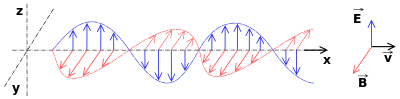
\includegraphics[height = 100pt, width = 300pt]{ondeEM.png}
\end{center}


\section{Cas particulier du vide (1D) : équations d'Alembert}

Nous allons traiter ici du \textit{cas particulier du \textbf{vide}} en une seule dimension spatiale.  \\
C'est à dire que nous allons considérer que le champ électrique ne dépend que d'une seule variable spatiale et du temps et pointe dans une seule direction (qui n'est pas celle de la variable pour éviter la confusion par après).
Nous écrivons alors $\vec{E}(x,y,z,t) \Rightarrow \vec{E_{y}}(x,t)$. \\Il en est de même pour le champ magnétique d'excitation (ou d'induction) nous considérons qu'il est 
\textit{orthogonal} au champ électrique et dépend aussi de $x$ et $t$ seulement ; $\vec{H}(x,y,z,t) \Rightarrow \vec{H_{z}}(x,t)$. \\ 

\begin{itemize}
	\item
Soit nous repartons de ce que nous avons déjà fait pour le cas général, l'équation d'onde est alors immédiate. \\
En effet, en 1D, le \textbf{Laplacien} vectoriel de $\vec{E}$ donne simplement sa dérivée partielle seconde en son unique variable
spatiale : 
\[ \Delta \vec{E} = \mu_{0} \epsilon_{0}  \frac{\partial^{2} \vec{E}}{\partial t^{2}} \Rightarrow \frac{\partial^{2} \vec{E} }{\partial x^2} = \frac{1}{c^{2}}  \frac{\partial^{2} \vec{E}}{\partial t^{2}}\]
qui se résout de manière \textit{scalaire} pour la direction unitaire de la variable ($y$ par exemple ici) : 
\[\frac{\partial^{2} E_{y}}{\partial x^{2}} = \frac{1}{c^{2}}  \frac{\partial^{2} E_{y}}{\partial t^{2}}\]


\item Soit nous repartons de zéro et adoptons une méthode plus \textit{faible} mathématiquement parlant et faisons les hypothèses suivantes.\\
Nous admettrons pour ce qui suit que la matrice \textit{Hessienne} des uniques fonctions scalaires liées à $\vec{E}$ et $\vec{H}$ soit symétrique. 
Plus particulièrement, nous pouvons imposer que ces fonctions soient de classe $\mathcal{C}^{2}$ ce qui vérifie la condition sur la \textit{Hessienne}. \\ 

Nous pouvons dès lors écrire, tout en se basant sur les équations de Maxwell : 


\begin{equation*}
	\begin{split}
\nabla \times \vec{E} =& -\mu_{0} \frac{\partial \vec{H}}{\partial t} \\=& (\frac{\partial E_{z}}{\partial y} - \frac{\partial E_{y}}{\partial z})\hat{x} +   (\frac{\partial E_{x}}{\partial z} - \frac{\partial E_{z}}{\partial x})\hat{y} +
(\frac{\partial E_{y}}{\partial x} - \frac{\partial E_{x}}{\partial y})\hat{z} \\=& \frac{\partial E_{y}}{\partial x} \hat{z}
	\end{split}
\end{equation*}
\begin{equation*}
\begin{split}
\nabla \times \vec{H} &= \epsilon_{0} \frac{\partial \vec{E}}{\partial t} \\&= (\frac{\partial H_{z}}{\partial y} - \frac{\partial H_{y}}{\partial z})\hat{x} +   (\frac{\partial H_{x}}{\partial z} - \frac{\partial H_{z}}{\partial x})\hat{y} +
(\frac{\partial H_{y}}{\partial x} - \frac{\partial H_{x}}{\partial y})\hat{z} \\&= -\frac{\partial H_{z}}{\partial x} \hat{y}
	\end{split}
\end{equation*}

Nous possédons alors un système d'EDP linéaires couplées deux à deux de premier ordre. \\
La résolution de ce genre de système est un problème typique lié aux \textit{équations aux dérivées partielles} et est abordé dans le cours
de mathématiques 3. Nous allons ici transformer ce système en deux EDP linéaires de second ordre dont la résolution est semblable. \\
Nous pouvons dériver la première équation ci-dessus par rapport à $x$ et la seconde par rapport au temps $t$ : 

\[  \frac{\partial^{2} \vec{H}}{\partial x \partial t} = -\frac{1}{\mu_{0}} \frac{\partial^{2} E_{y}}{\partial x^{2}} \hat{z}\]
\[  \frac{\partial^{2} H_{z}}{\partial t \partial x} \hat{y} = - \epsilon_{0} \frac{\partial^{2} \vec{E}}{\partial t^{2}} \]

Comme les dérivées partielles secondes sont \textit{croisées} et si nous travaillons en termes de \textbf{\textit{normes}} :

\[\frac{\partial^{2} E_{y}}{\partial x^{2}} = \frac{1}{c^{2}}  \frac{\partial^{2} E_{y}}{\partial t^{2}} \hspace{10pt} \mbox{||} \hspace{10pt} \frac{\partial^{2} H_{z}}{\partial x^{2}} = \frac{1}{c^{2}}  \frac{\partial^{2} H_{z}}{\partial t^{2}}\]
\end{itemize}

\textit{Les EPD de second ordre linéaires homogènes en 1D (et temps) de type hyperbolique} admettent une solution générale du type\footnote{A nouveau, se référer au cours de Mathématiques 3}  : 
$ \xi(x,t) = \frac{1}{2}(f(x-ct)+f(x+ct)) $. \\ 
Dans le cas d'ondes, nous travaillerons souvent avec des fonctions $f$ sinusoïdales admettant parfois un déphasage $\phi$ çà et là. 
 

\section{Propriétés des EDP linéaires couplées de premier ordre (1D et temps)}

De manière tout à fait générale, si deux grandeurs \textit{scalaires} A et B dépendant d'une variable temporelle et une variable spatiale sont 
liées par des équations de type 

\[\frac{\partial A}{\partial x} = -\alpha \frac{\partial B}{\partial t}\]

\[\frac{\partial A}{\partial t} = -\beta \frac{\partial B}{\partial x}\]

elles \textbf{obéissent toutes deux à une même équation d'onde de type} : $\frac{1}{c^{2}} \frac{\partial^{2} A,B}{\partial t^{2}} = \frac{\partial^{2} A,B}{\partial x^{2}}$. 
Le paramètre $c$ représente toujours la \textit{vitesse} de propagation de la grandeur scalaire et vaut : $c = \sqrt{\frac{\beta}{\alpha}}$. 
Le rapport entre ces deux grandeurs est nommé \textit{impédance caractéristique} et vaut quant à elle : $\mathcal{Z} = \sqrt{\alpha\beta}$.\footnote{Les grands voyageurs parmi vous auront immédiatement reconnu la fameuse enseigne grecque :\\ le supermarché low-cost Alpha-Beta}\\ 

Nous pouvons prouver l'existence d'un tel $\mathcal{Z}$ comme marqué dans les slides. Soient donc deux solutions à l'équation d'onde et aux équations couplées données par les expressions suivantes :

\[S_{1}(x,t) = \mathcal{F}(x-ct) + \mathcal{F}(x+ct)\]
\[S_{2}(x,t) = \mathcal{G}(x-ct) + \mathcal{G}(x+ct)\]

Si nous posons $w = x-ct$ et $u = x+ct$ nous pouvons écrire grâce aux équations couplées : 
\begin{fullwidth}
	\[\frac{\partial S_{1}}{\partial x} = -\alpha \frac{\partial S_{2}}{\partial t} \Leftrightarrow \frac{\partial \mathcal{F}(w)}{\partial w}\frac{\partial w}{\partial x} + \frac{\partial \mathcal{F}(u)}{\partial u}\frac{\partial u}{\partial x} 
	= -\alpha (\frac{\partial \mathcal{G}(w)}{\partial w}\frac{\partial w}{\partial t} + \frac{\partial \mathcal{G}(u)}{\partial u}\frac{\partial u}{\partial t})\]
	
	\[\frac{\partial S_{1}}{\partial t} = -\beta \frac{\partial S_{2}}{\partial x} \Leftrightarrow \frac{\partial \mathcal{F}(w)}{\partial w}\frac{\partial w}{\partial t} + \frac{\partial \mathcal{F}(u)}{\partial u}\frac{\partial u}{\partial t} 
	= -\beta (\frac{\partial \mathcal{G}(w)}{\partial w}\frac{\partial w}{\partial x} + \frac{\partial \mathcal{G}(u)}{\partial u}\frac{\partial u}{\partial x})\]
\end{fullwidth}	
	En simplifiant les équations : 
\begin{fullwidth}	
	\begin{equation}
	\frac{\partial \mathcal{F}(w)}{\partial w} + \frac{\partial \mathcal{F}(u)}{\partial u}
	= -\alpha (-c \frac{\partial \mathcal{G}(w)}{\partial w} + c \frac{\partial \mathcal{G}(u)}{\partial u}) \Rightarrow
	\frac{\partial \mathcal{F}(w)}{\partial w} + \frac{\partial \mathcal{F}(u)}{\partial u} = -\alpha c (-\frac{\partial \mathcal{G}(w)}{\partial w} +\frac{\partial \mathcal{G}(u)}{\partial u}) 
	\end{equation}
	
	\begin{equation}
	-c \frac{\partial \mathcal{F}(w)}{\partial w} + c \frac{\partial \mathcal{F}(u)}{\partial u}
	= -\beta (\frac{\partial \mathcal{G}(w)}{\partial w} + \frac{\partial \mathcal{G}(u)}{\partial u}) \Rightarrow -\frac{\partial \mathcal{F}(w)}{\partial w} + \frac{\partial \mathcal{F}(u)}{\partial u}
	= -\frac{\beta}{c} (\frac{\partial \mathcal{G}(w)}{\partial w} + \frac{\partial \mathcal{G}(u)}{\partial u})
	\end{equation}
\end{fullwidth}	

En additionnant les équations (5) et (6), et en définissant $\mathcal{Z} = \frac{\beta}{c} = \alpha c$ nous obtenons : 

\begin{equation}
 \frac{\partial \mathcal{F}(u)}{\partial u} =  \mathcal{Z} \frac{\mathcal{G}(u)}{\partial u}
\end{equation}

Ce qui donne, après intégration (le résultat est exactement symétrique pour le cas $\mathcal{F}(w), \mathcal{G}(w)$) 

\[\mathcal{F}(u) = \mathcal{Z} \cdot \mathcal{G}(u) + \mathcal{K}\]

Si nous considérons des \textbf{phénomènes physiques} de \textit{propagation}, la constante $\mathcal{K}$ est tout simplement nulle car 
à l'origine, la propagation n'a pas encore eu lieu. 


Etant donnée la symétrie des équations, nous pouvons tirer la même conclusion quant aux grandeurs $\mathcal{S}_{1},\mathcal{S}_{2}$. 
Immédiatement, il vient que l'\textit{impédance caractéristique} d'une onde\\ électromagnétique en considérant le vecteur $\vec{J}$ nul vaut 
$\mathcal{Z} = \sqrt{\frac{\mu}{\epsilon}} \simeq120 \pi \simeq 377 [\Omega] $. 

\section{Représentation du cas particulier 1D}

Etant donné que nous avons pu caractériser l'équation d'onde du cas particulier et en tirer certaines conclusions, 
voici donc la forme générale du champ électrique d'une \textit{onde EM plane monochromatique} (\textit{polarisée linéairement}, nous y reviendrons).

\[\vec{E}(x,y,z,t) \Rightarrow \vec{E}_{y}(x,t) = \xi sin(k x - \omega t + \phi) \hat{y} \]
où $\xi,\omega,t,k,x,\phi$ sont respectivement l'élongation maximale en chaque point de l'espace, la \textit{pulsation} (la fréquence  vaut $f = \frac{w}{2 \pi} = \frac{2\pi}{T}$ où $T$ 
est la période du signal), le temps, le nombre d'onde ($k = \frac{2\pi}{\lambda}$ où $\lambda$ est la longueur d'onde), la position sur l'axe des X, le déphasage  du champ électrique. 
\begin{marginfigure}
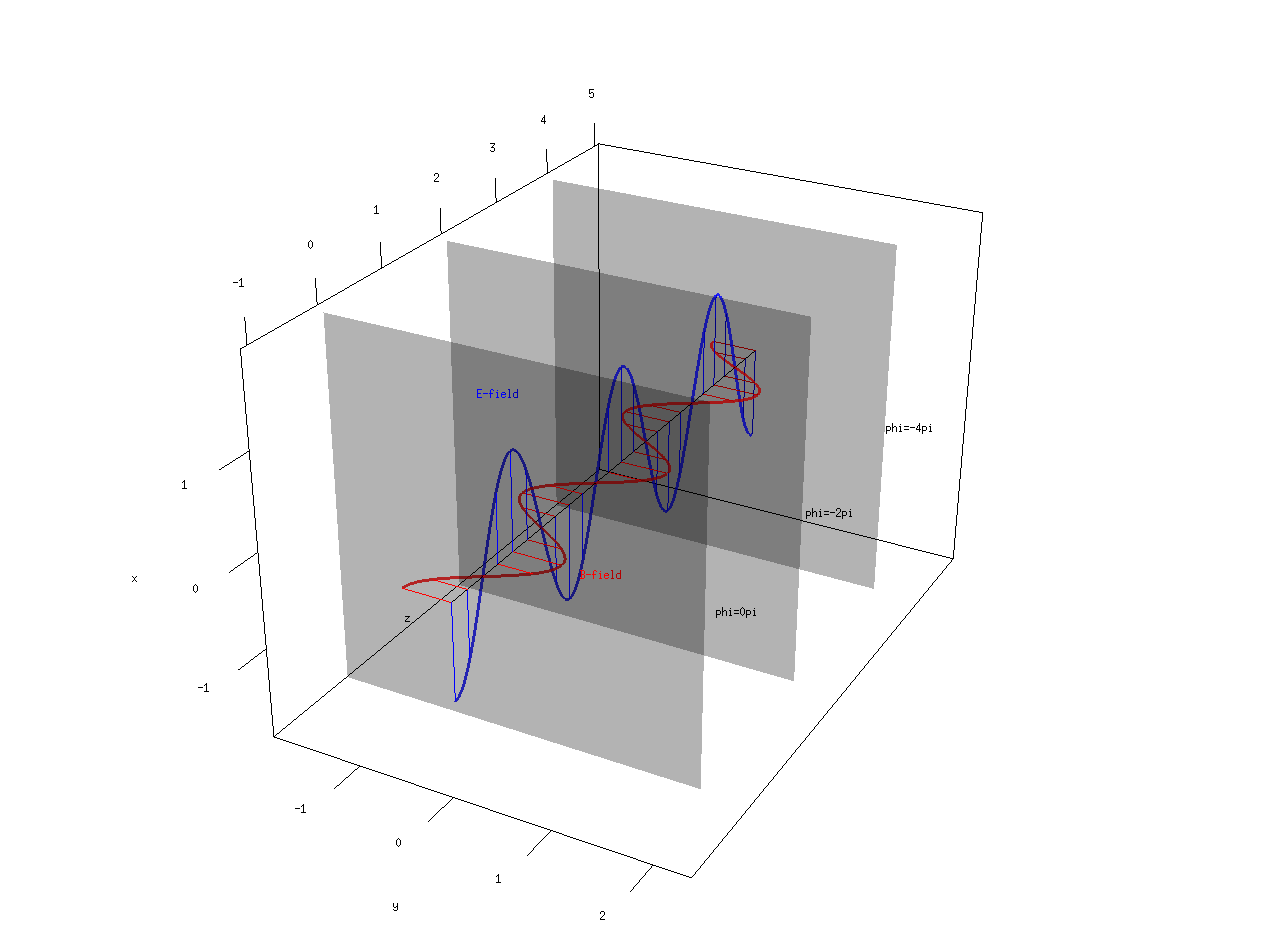
\includegraphics[width = \linewidth]{onde.png}
\caption{\textit{\textbf{Représentation d'une onde EM plane monochromatique polarisée linéairement ($\vec{E}$ vers $\hat{x}$).}}}
\end{marginfigure}




\section{Intensité d'une onde EM}  %%%%% /!\ PROFESSEURS : Avez-vous une démonstration plus complète que les slides quant à l'intensité d'une onde EM?

% AUTEUR :: Brieuc Pinon || SOURCE ::  YOUNG 13th p.1176->1178 || DATE :: 18.10.15
Quelle énergie transporte une onde électromagnétique?

Pour rappel les densités d'énergie dans le vide associées au magnitudes des champs électrique et magnétique sont 
\[u=\frac{1}{2}\epsilon_0E^{2}\]
\[u=\frac{\mu_0H^{2}}{2}\]

On sait que $\mu_0H=\frac{E}{c}=\sqrt{ \epsilon_0 \mu_0 }E$ dans le vide. On en déduit en sommant les énergies électrique et magnétique
\[u=\frac{1}{2}\epsilon_0E^{2} + \frac{1}{2\mu_0}(\sqrt{ \epsilon_0 \mu_0 }E)^{2} = \epsilon_0E^{2}\]

On remarque que les énergies associées aux champs électrique et magnétique sont égales dans notre onde.

L'énergie transportée par une onde électromagnétique peut être exprimée en fonction de la densité d'énergie, de sa vitesse et de la surface qu'elle traverse comme suit (avec A la surface perpendiculaire au déplacement de l'onde et c la célérité)
\[dU=udV=(\epsilon_0E^{2})Ac dt\]

Que l'on peut écrire sous forme d'un débit d'énergie par seconde par unité de surface (soit des $\frac{W}{m^{2}}$), que l'on appelle S
\[S=\frac{1}{A}\frac{dU}{dt}=\epsilon_0cE^{2}\]
ou en substituant $c$ par $1/\sqrt{\epsilon_0 \mu_0}$
\[S=\frac{EB}{\mu_0}\]

\begin{figure}
	\centering
	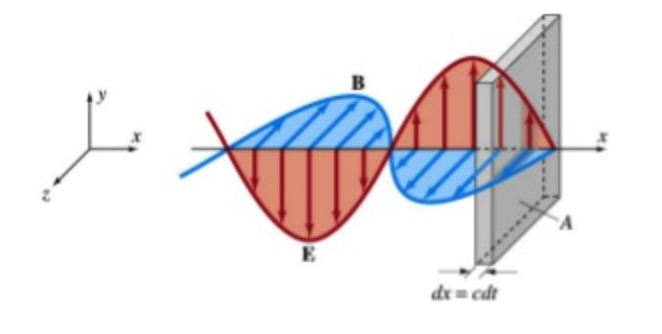
\includegraphics[height = 80pt, width = 200pt]{poynting.png}
	\caption{Vecteur de Poynting}
	\label{poynting}
\end{figure}

Afin de pouvoir l'utiliser en pratique avec des surfaces, on doit le définir sous forme d'un vecteur dont la direction et le sens sont ceux de propagation. On choisit évidemment $S$ comme norme.
\[\vec{S}=\vec{E} \times \vec{H} \]
Ce vecteur est le vecteur de \textit{\textbf{Poynting}} (vecteur \textit{normal} au pavé : voir figure \ref{poynting}), ici défini dans le vide.
Ce nouveau vecteur nous permet de définir la puissance passant à travers une surface comme
\[P=\oint_{S}\vec{S} \cdot d\vec{A}\] %%%% /!\ PROFESSEURS le Young prend une surface fermée mais ça ne parait pas très générale comme expression, l'expression est-elle correcte pour une surface ouverte?

Cette expression n'est pas encore très pratique en application directe car nos champs électromagnétiques varient dans le temps (faut-il le rappeler?). La moyenne de $S$ parait un choix plus judicieux dans nos applications, nous appelons cette moyenne l'intensité de l'onde électromagnétique. L'intensité dépend de la fonction d'onde dans le cas  d'une fonction sinusoïdale, nous obtenons (rappel: $\int_0^{2\pi} \sin^{2}(x) \, dx = \frac{1}{2}$)

\[I_{moy} = S_{av} = \frac{ E_{max} H_{max}}{2} = \frac{E_{max}^{2}}{2\mu_0c} = \frac{1}{2} \sqrt{\frac{\epsilon_0}{\mu_0}} E_{max}^{2} = \frac{1}{2}\epsilon_0 c E_{max}^{2}\]
toujours en $\frac{W}{m^{2}}$.

Tous les résultats peuvent facilement être adaptés dans des milieux de propagation non-vides. Il est nécessaire d'appliquer les substitutions $\epsilon_0 \rightarrow \epsilon$, $\mu_0 \rightarrow \mu$ et $c \rightarrow v $.\\

%%%% COMMENT écrire directement sous cette forme les équations?


%%%%%/!\ COMMENT cette partie est en doublon supprimer/fusionner? 
%%%%% /!\  OUI effectivement :) 
%Nous n'avons malheureusement pas trouvé de démonstration %convaincante à ce sujet. \\
%Pour rappel, nous définissons que l'\textit{intensité %maximale} d'une onde EM, c'est à dire 
%le produit de sa densité d'énergie maximale par sa vitesse, vaut ....

Notons encore que dans certains exercices, il peut être intéressant de connaitre la valeur maximale à l'instant $t$ de cette intensité. Elle vaut simplement le double de $I_{moy}$ si la fonction d'onde concernée est de type \textit{sinuosïdale}. 

\[I_{max} = \epsilon c E_{max}^{2} = \sqrt{\frac{\epsilon}{\mu}}E_{max}^{2} = \sqrt{\frac{\mu}{\epsilon}}H_{max}^{2} = E_{max} H_{max} \hspace{5pt} [W/m^{2}]\]


% Etant donné que la moyenne d'un sinus au carré (car $\vec{E}$ %et $\vec{H}$ sont très souvent exprimés de cette manière) %vaut $\frac{1}{2}$

%\[I_{moy} = \epsilon c \frac{E_{max}^{2}}{2} = %\sqrt{\frac{\epsilon}{\mu}}\frac{E_{max}^{2}}{2} = %\sqrt{\frac{\mu}{\epsilon}}\frac{H_{max}^{2}}{2} = ù\frac{E_{max} H_{max}}{2} \hspace{5pt} [J/m^{2}]\] 
